\begin{frame}{Precision estimates at the LHC}
  \framesubtitle{Evidence for Beyond-Standard-Model physics}

  \begin{columns}

    \begin{column}{0.5\textwidth}

      \begin{figure}
        \centering
        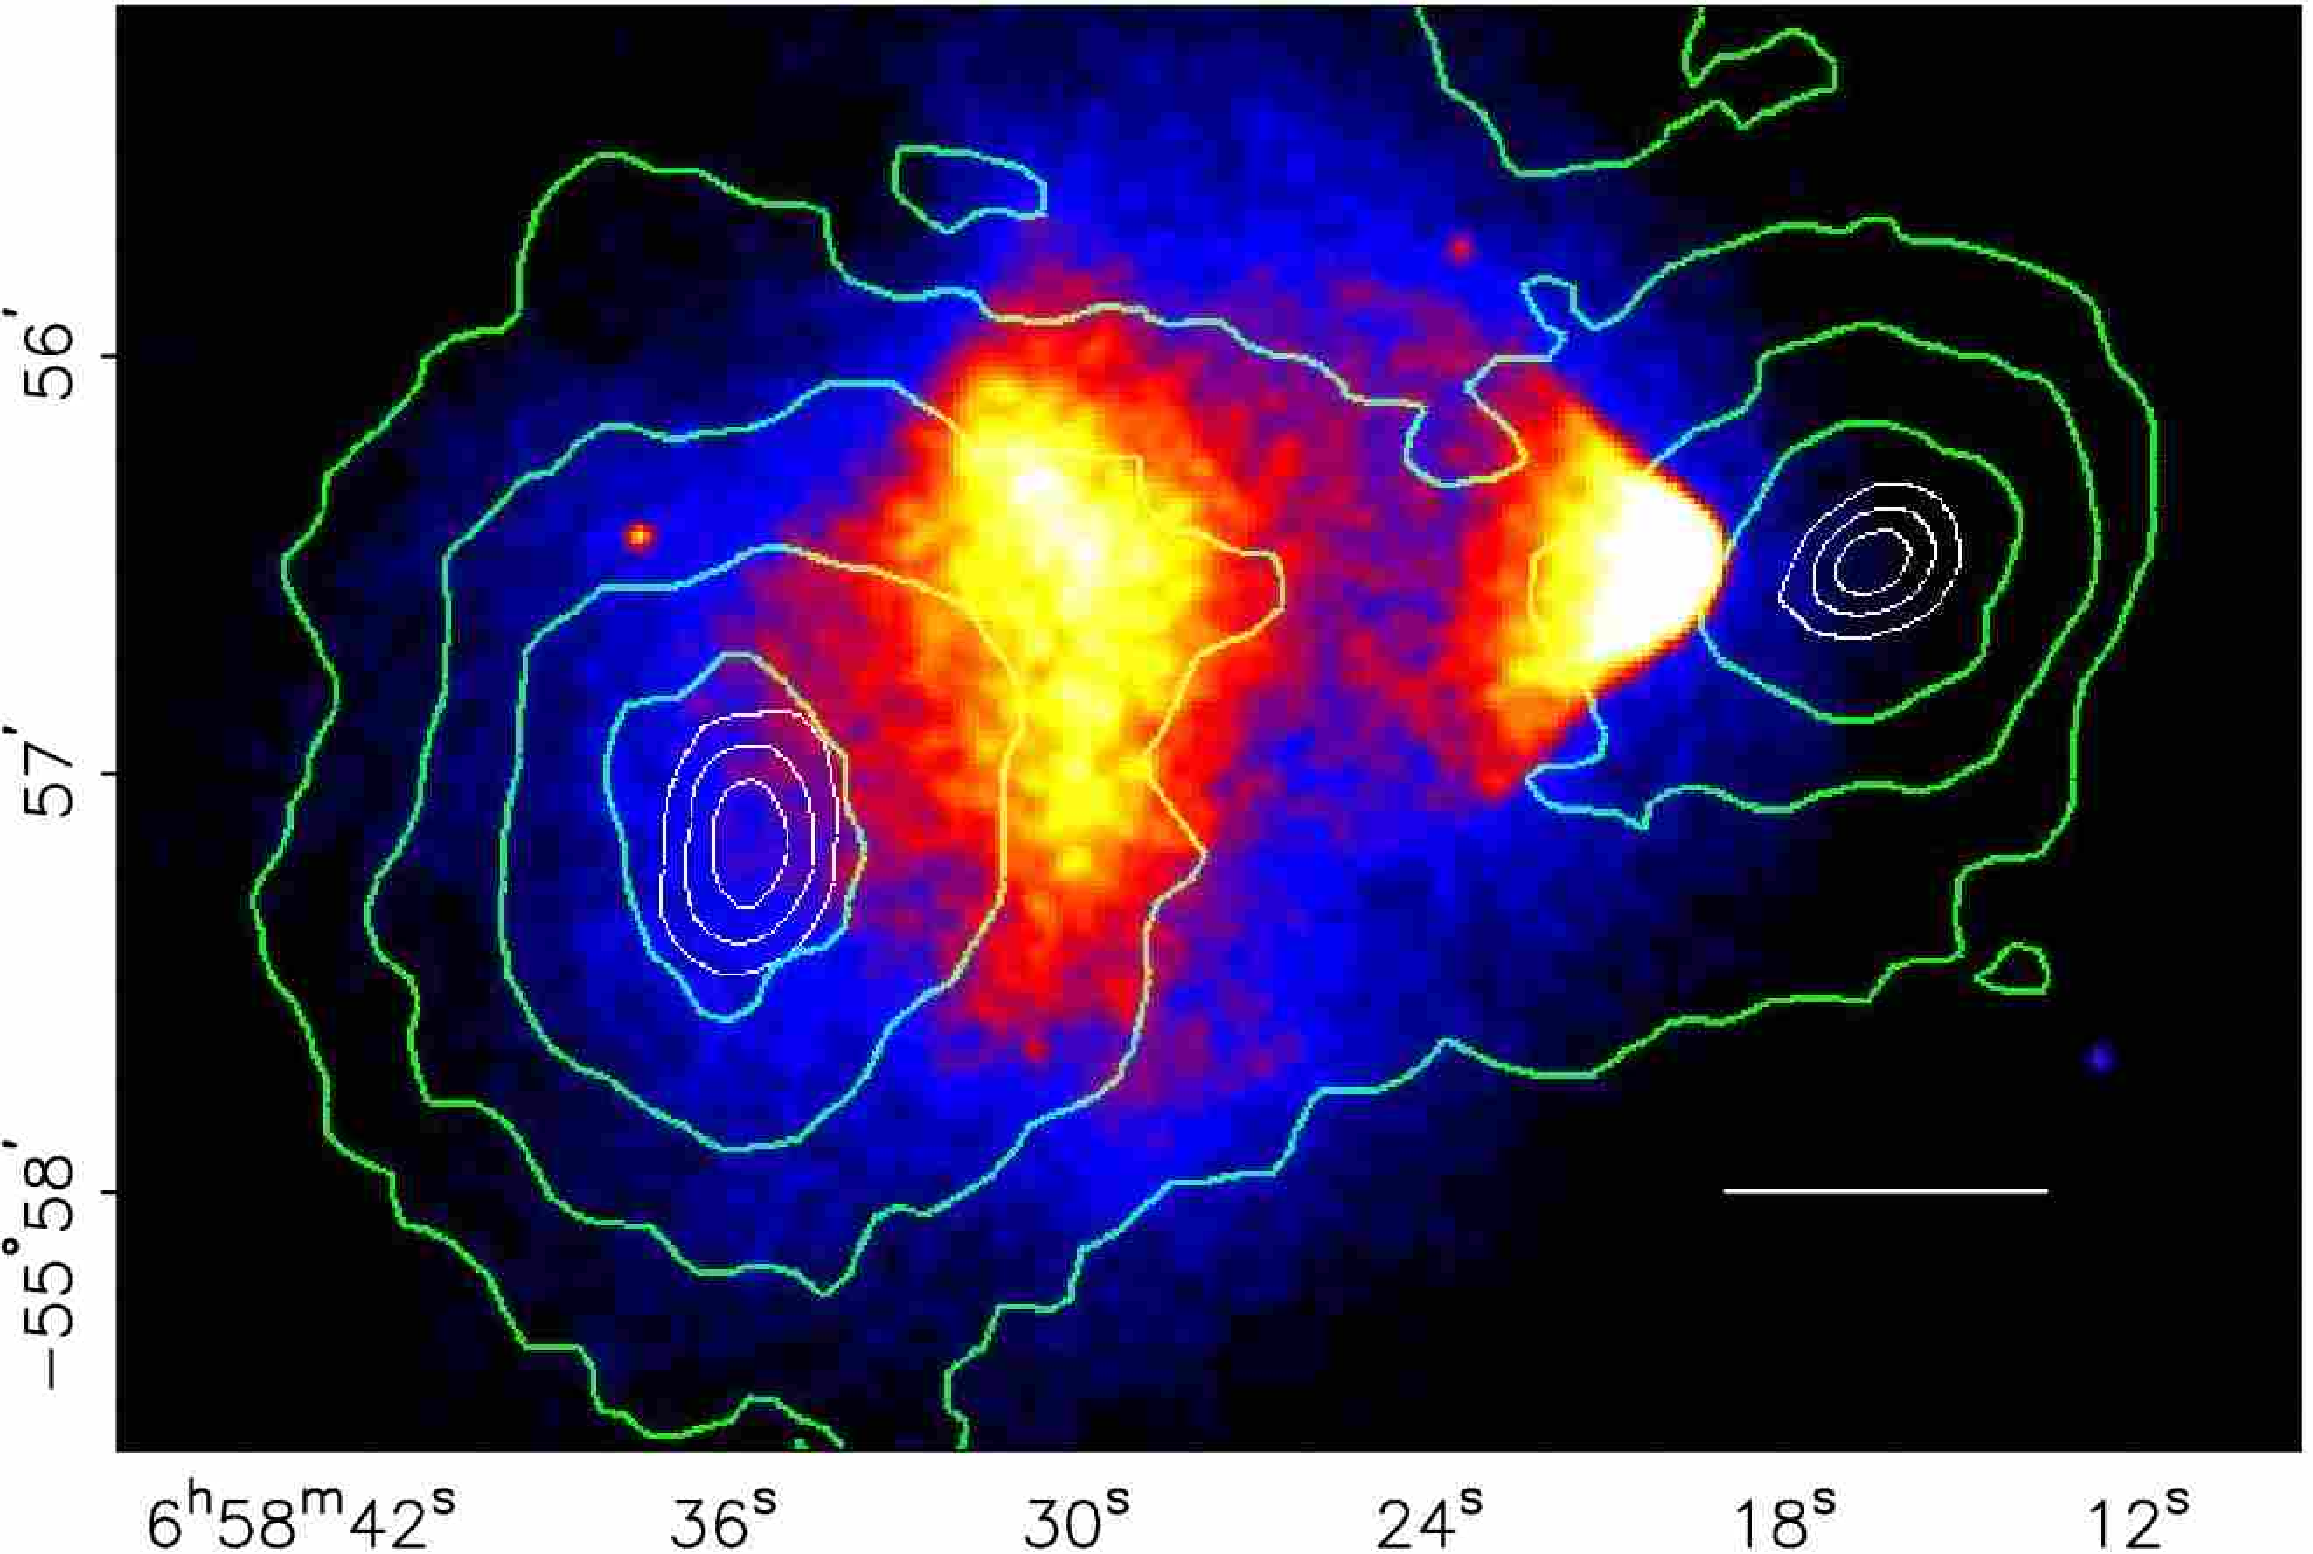
\includegraphics[width = \textwidth]{imgs/clowe-2.png}
      \end{figure}

    \end{column}

    \begin{column}{0.5 \textwidth}

      \begin{colorblock}[black]{statalegrey}{Main BSM evidence}
        \begin{itemize}
          \item dark matter and dark energy
          \item matter-antimatter asymmetry
          \item neutrino masses
        \end{itemize}
      \end{colorblock}

      \vspace{0.5em}

      \capcol{Figure} from Clowe et al. 2006.

      \justifying
      Offset between the observed baryonic mass distribution and the gravitational potential in the Bullet Cluster (1E 0657-56).

    \end{column}

  \end{columns}

\end{frame}

%=======================================================================

\begin{frame}{Precision estimates at the LHC}
  \framesubtitle{BSM constraints and shift in research paradigm}

  \begin{columns}

    \begin{column}{0.5 \textwidth}

      \begin{colorblock}[black]{statalegrey}{Main BSM proposals}
        \begin{itemize}
          \item supersymmetric models (MSSM, \dots)
          \item dark matter models (WIMPs, axions, \dots)
          \item extended gauge sectors ($ \mathrm{SO}(10) $, \dots)
          \item SM Effective Field Theory (SMEFT)
        \end{itemize}
      \end{colorblock}

      \vspace{0.5em}

      \capcol{Figure} from ATLAS PUB Note 2023--025.

      \justifying
      Exclusion limits in the $ \tilde{g} - \tilde{\chi}^0_1 $ mass plane for various models for the decay of the gluino to the lightest supersymmetric particle.

    \end{column}

    \begin{column}{0.5\textwidth}

      \begin{figure}
        \centering
        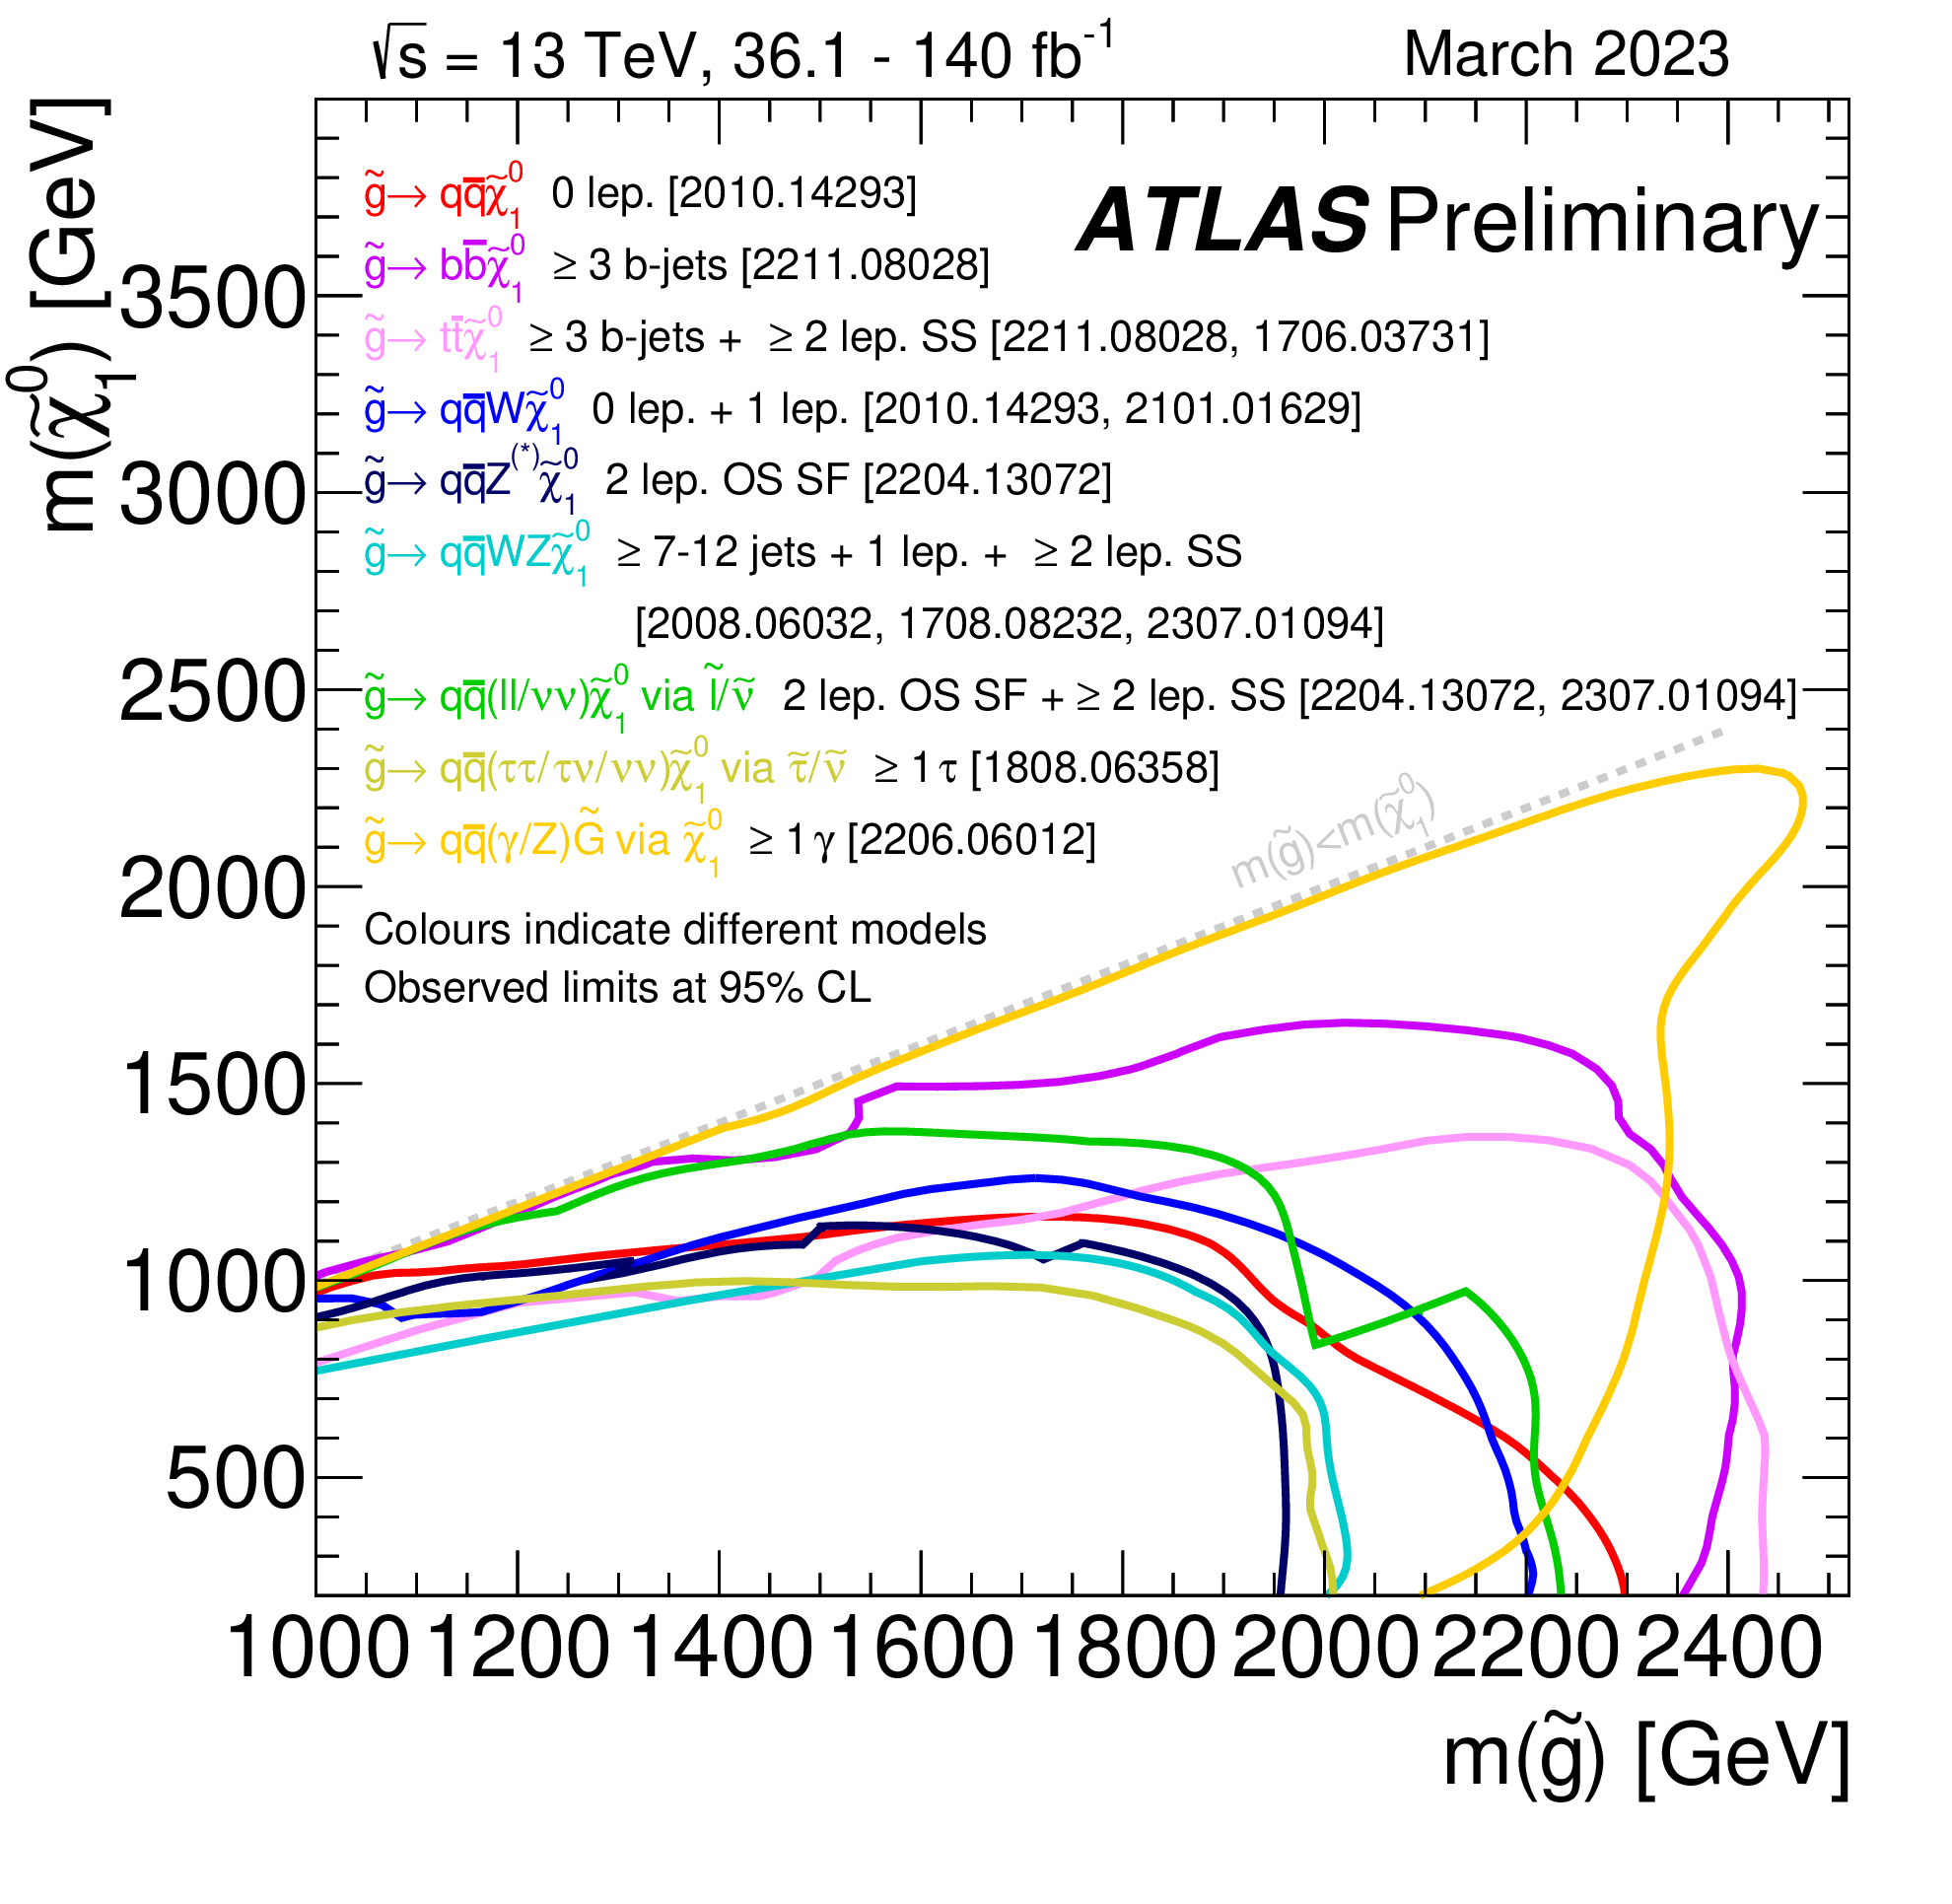
\includegraphics[width = 0.94\textwidth]{imgs/susy.png}
      \end{figure}

    \end{column}

  \end{columns}

\end{frame}

%=======================================================================

\begin{frame}{Precision estimates at the LHC}
  \framesubtitle{Factorization theorem and perturbative QCD}

  \begin{columns}

    \begin{column}{0.5 \textwidth}

      \begin{figure}
        \centering
        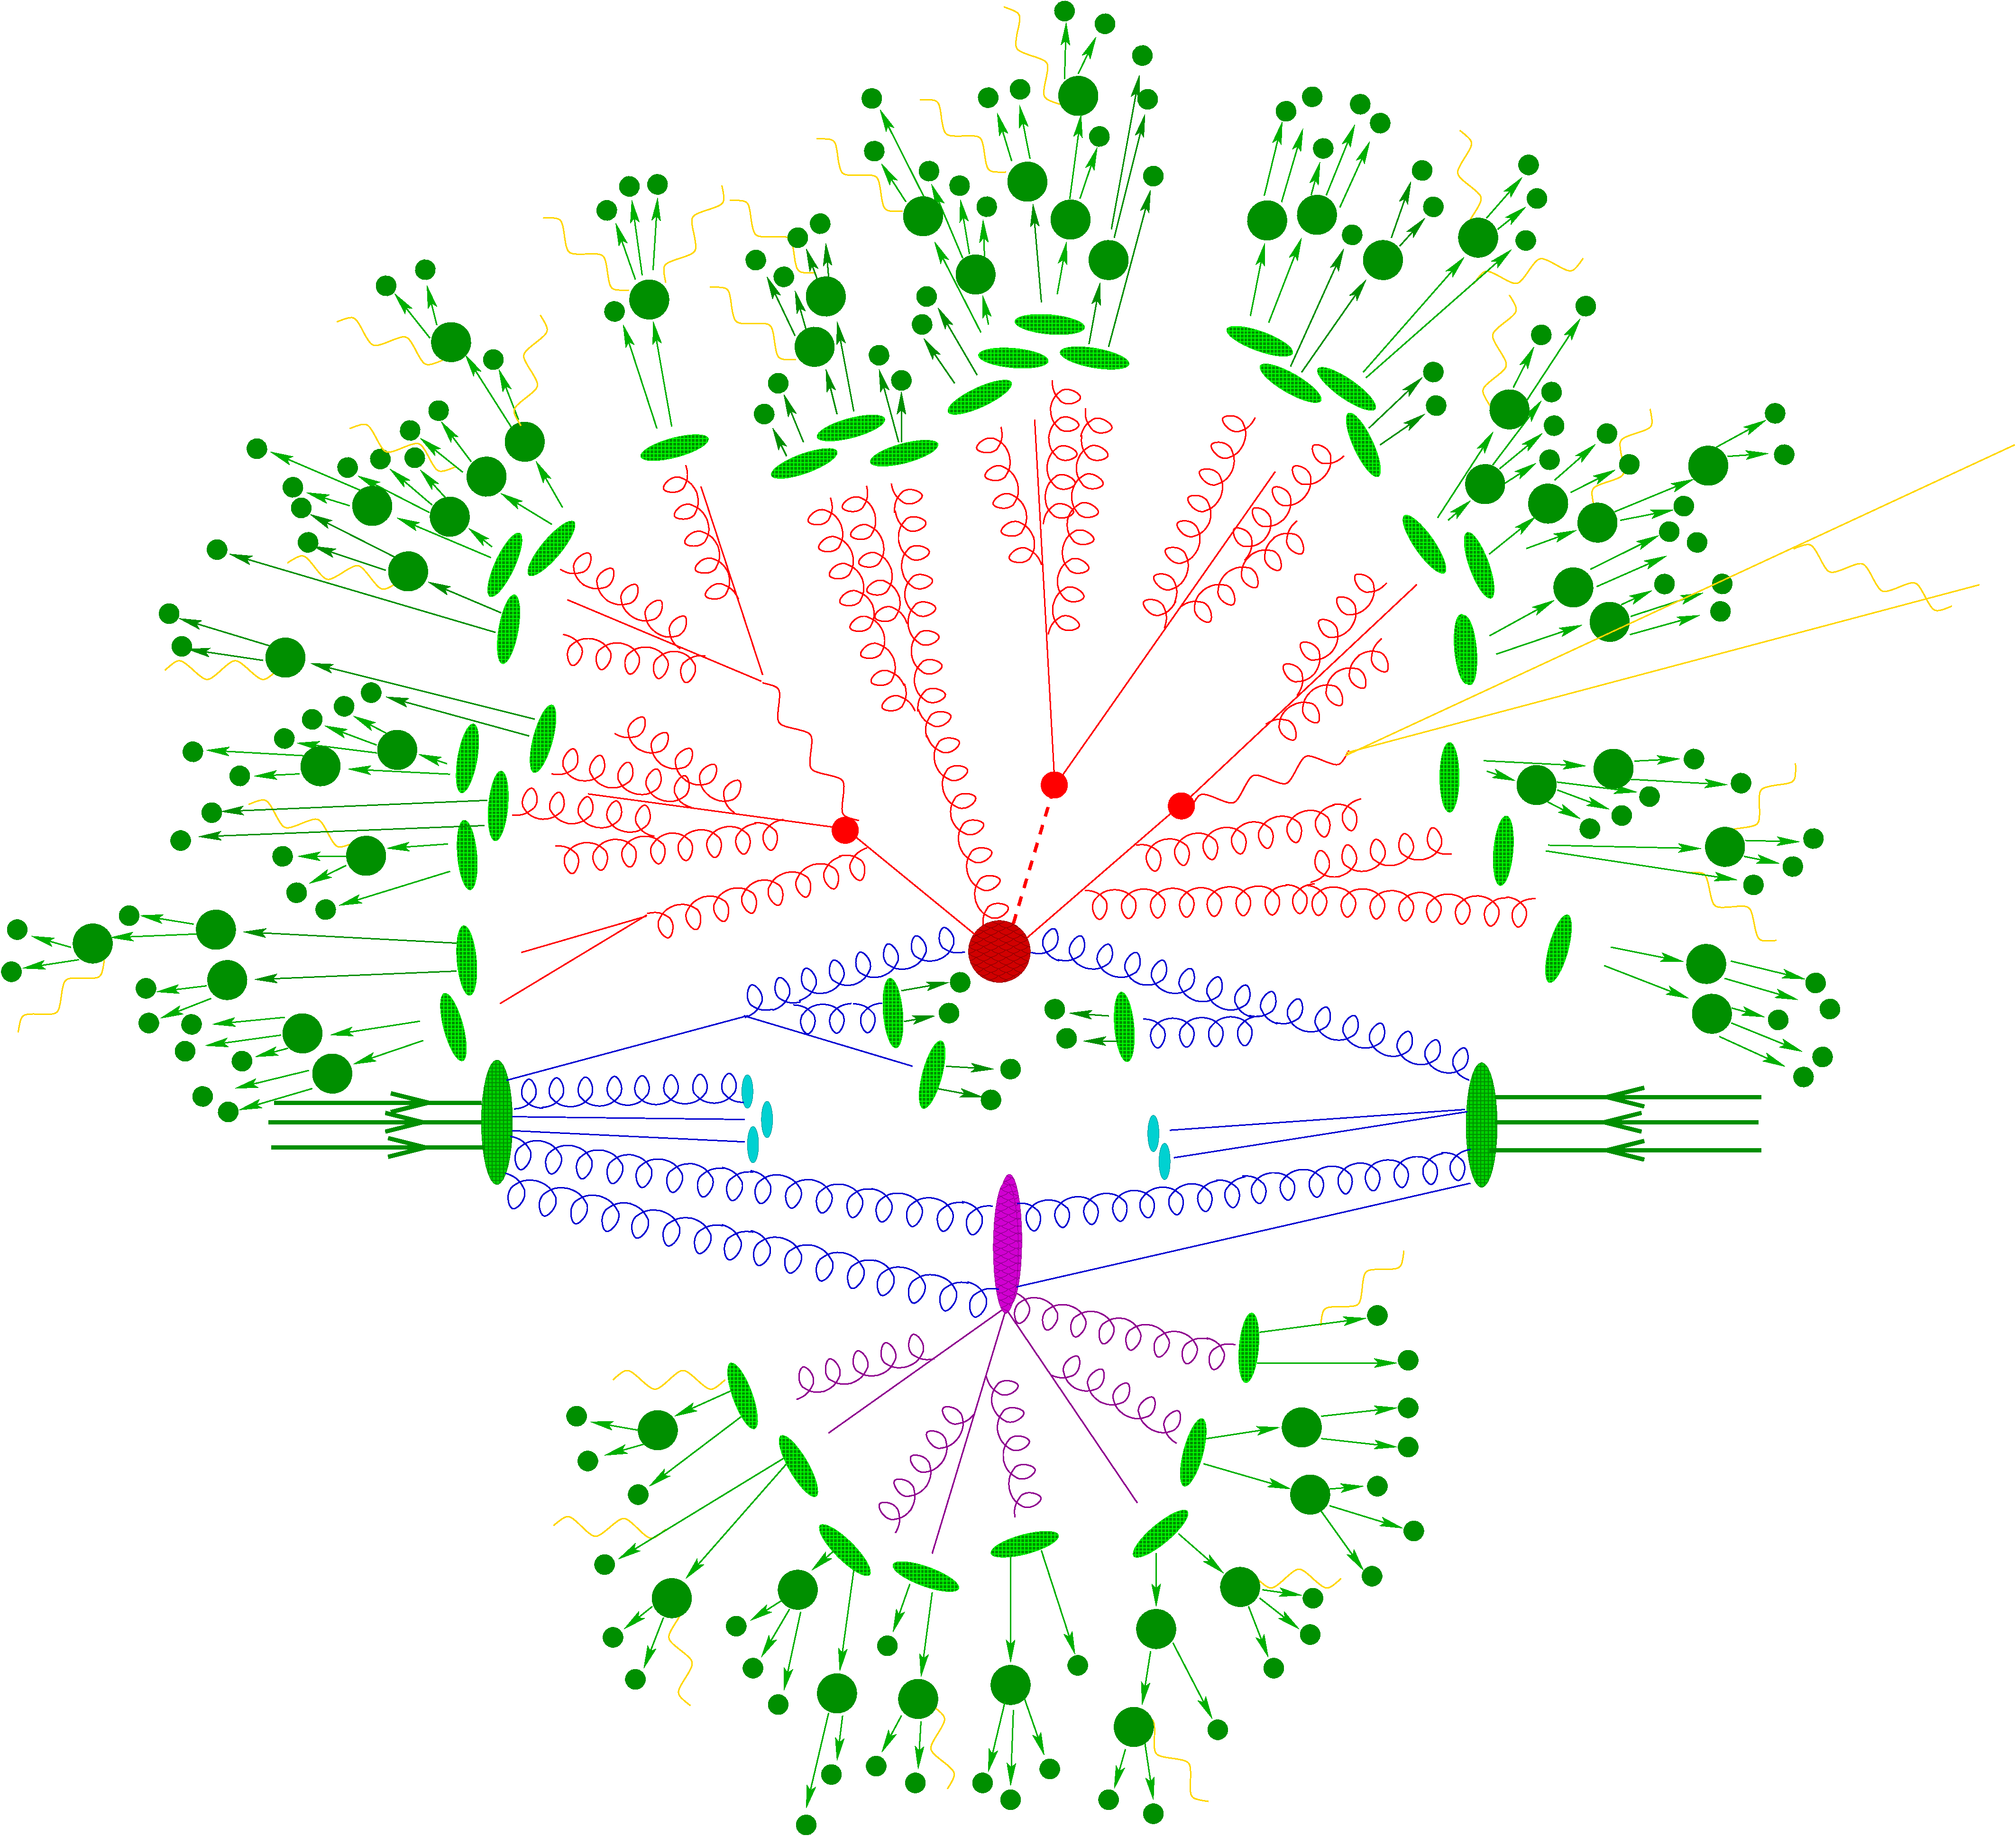
\includegraphics[width = \textwidth]{../imgs/hadr-scatt.pdf}
      \end{figure}

    \end{column}

    \begin{column}{0.5 \textwidth}

      \begin{figure}
        \centering
        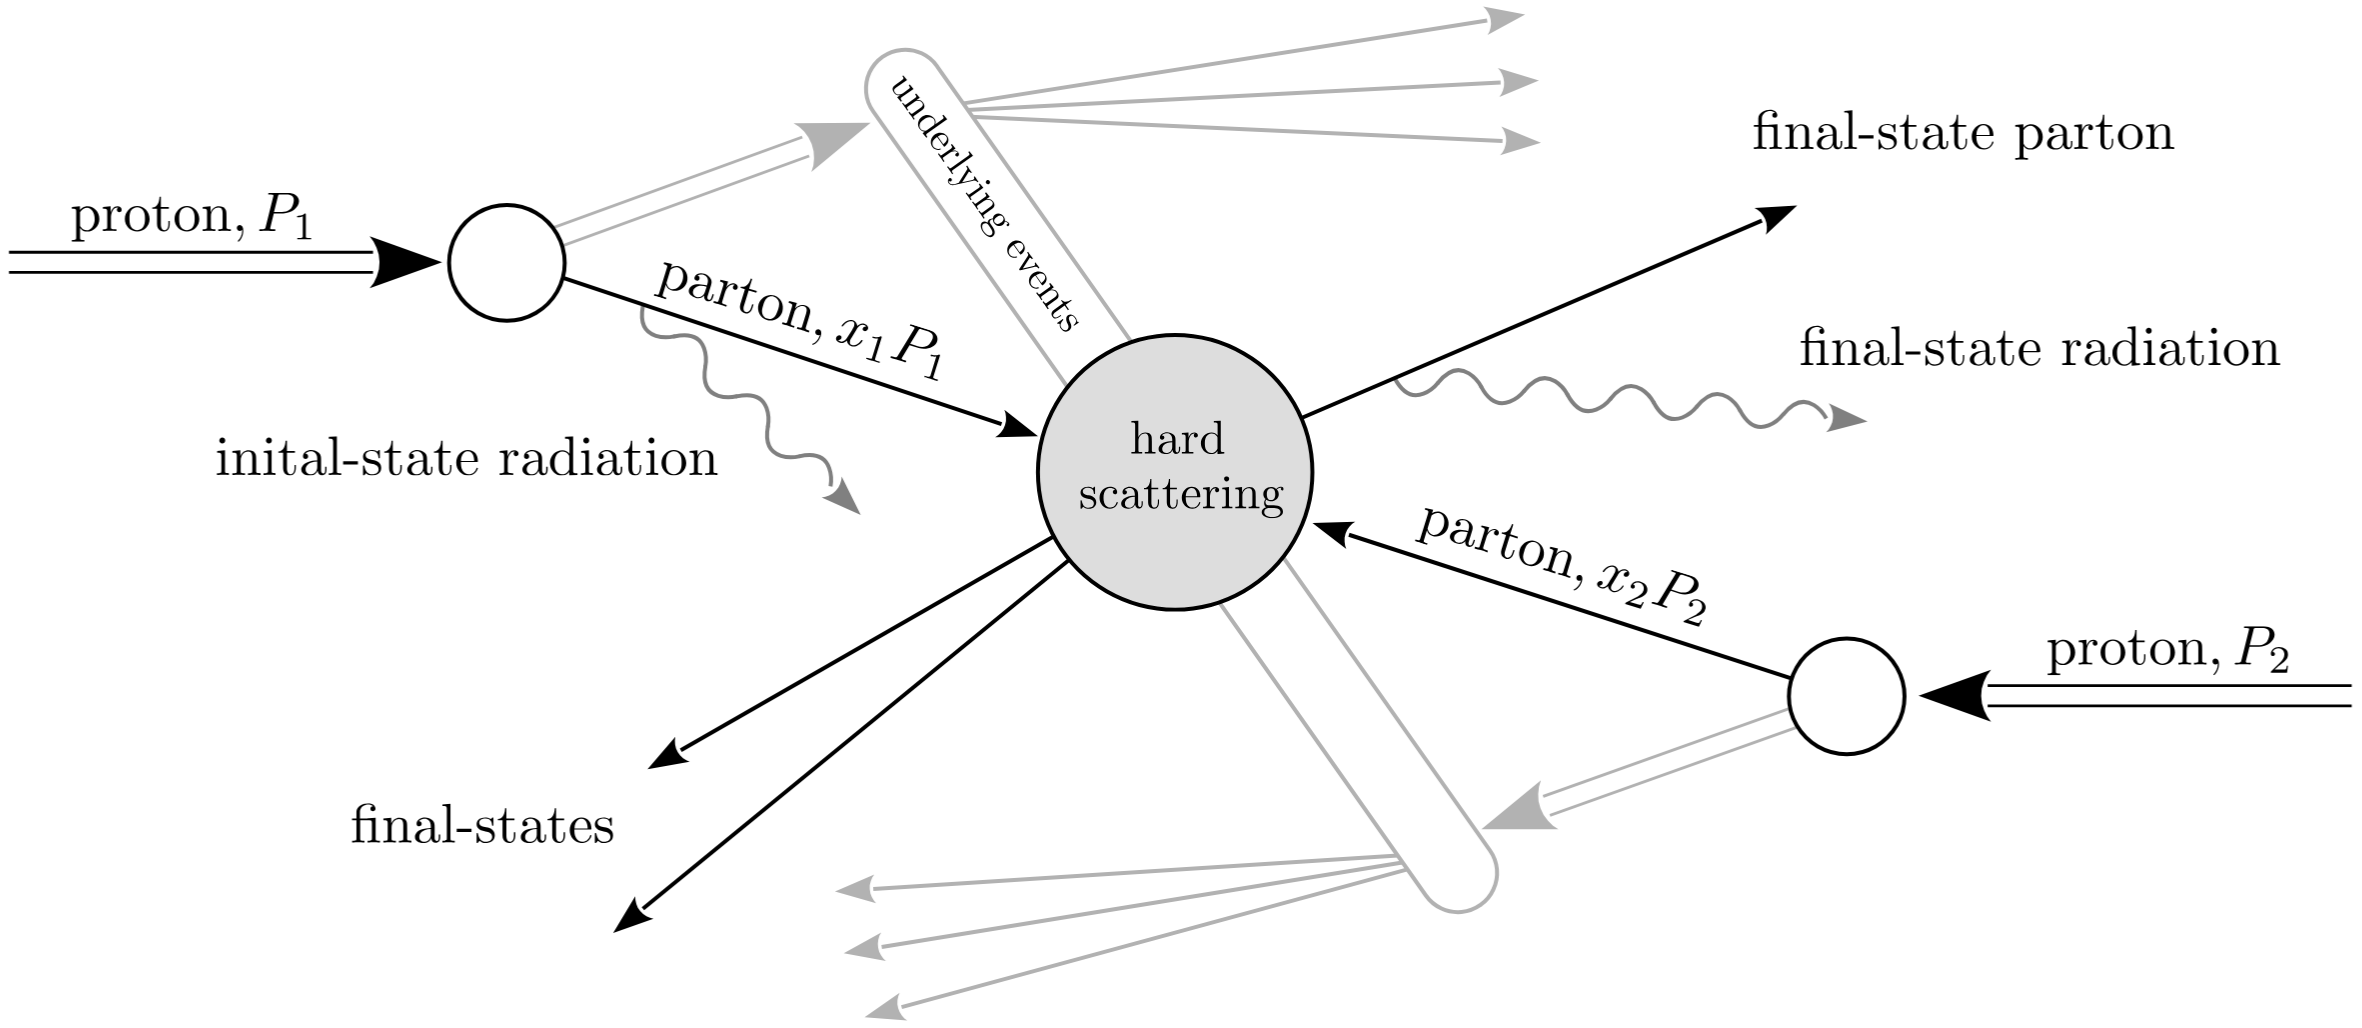
\includegraphics[width = \textwidth]{../imgs/part-scatt.png}
      \end{figure}

      \capcol{Figures} from Höche 2015 (left) and Asteriadis 2021 (right).

      \justifying
      Hadronization of jets produced in hadronic scattering and detail of the underlying hard partonic scattering.

    \end{column}

  \end{columns}

\end{frame}

%=======================================================================

\begin{frame}{Precision estimates at the LHC}
  \framesubtitle{Factorization theorem and perturbative QCD}

  \justifying
  Hadronic and partonic physics decouple in hard scattering processes, and we can formulate a factorization theorem:
  \begin{multline*}
    \dd\hcs_{h_1 , h_2}(P_1 , P_2) = \sum_{a,b} \int_{[0,1]^2} \frac{\dd \xi_1}{\xi_1} \frac{\dd \xi_2}{\xi_2} \,\pdfb{a}{h_1}(\xi_1, \fac^2) \,\pdfb{b}{h_2}(\xi_2, \fac^2) \times \\
    \times \dd\pcs_{a,b}(\xi_1 P_1, \xi_2 P_2, \rc, \ren^2, \fac^2)
    \left[ 1 + \smo \left( \frac{\qcd^n}{Q^n} \right) \right]
  \end{multline*}
  \emph{Asymptotic freedom} allows for a perturbative analysis of the hard partonic scattering:
  \begin{equation*}
    \dd\pcs_{a,b}(p_1 , p_2) = \sum_{n \in \N_0} \dd\pcs_{a,b}^{(n)}(p_1 , p_2)
  \end{equation*}
  $ n \ge 1 $ are denoted by N$ ^n $LO QCD corrections.

\end{frame}

%=======================================================================

\begin{frame}{IR-pole structure of QCD}
  \framesubtitle{Radiative corrections to partonic processes}

  \vspace{0.1em}

  Our focus is on NLO QCD corrections. Consider e.g. the Drell-Yan process:
  \begin{equation*}
    \begin{tikzpicture}
    \begin{feynman}

      \vertex (a1) {\(q\)};
      \vertex[below = 3cm of a1] (a2) {\(\bar{q}\)};

      \vertex[below = 1.5cm of a1] (b1) {};
      \vertex[right = 2.25cm of b1, dot] (v1) {};

      \vertex[right = 2.25cm of v1, dot] (v2) {};
      \vertex[right = 2.25cm of v2] (b2) {};

      \vertex[above = 1.5cm of b2] (a3) {$ \ell^- $};
      \vertex[below = 1.5cm of b2] (a4) {$ \ell^+ $};

      \diagram* {
	(a1) -- [fermion] (v1),
	(a2) -- [anti fermion] (v1),

        (v1) -- [photon, edge label = {$ \gamma^* / Z $}] (v2),

	(v2) -- [fermion] (a3),
	(v2) -- [anti fermion] (a4),
      };
    \end{feynman}
    \end{tikzpicture}
  \end{equation*}

  \centering
  LO process

\end{frame}

%=======================================================================

\begin{frame}[noframenumbering]{IR-pole structure of QCD}
  \framesubtitle{Radiative corrections to partonic processes}

  Our focus is on NLO QCD corrections. Consider e.g. the Drell-Yan process:
  \begin{equation*}
    \begin{tikzpicture}
    \begin{feynman}

      \vertex (a1) {\(q\)};
      \vertex[below = 3cm of a1] (a2) {\(\bar{q}\)};

      \vertex[below = 1.5cm of a1] (b1) {};
      \vertex[right = 2.25cm of b1, dot] (v1) {};

      \vertex[right = 2.25cm of v1, dot] (v2) {};
      \vertex[right = 2.25cm of v2] (b2) {};

      \vertex[above = 1.5cm of b2] (a3) {$ \ell^- $};
      \vertex[below = 1.5cm of b2] (a4) {$ \ell^+ $};

      \vertex[dot , red] (c1) at ($(a1) + (1.5,-1)$) {};
      \vertex (c2) at ($(c1) + (1.5,1)$) {\color{red} $ g $};

      \diagram* {
	(a1) -- [fermion] (v1),
	(a2) -- [anti fermion] (v1),

        (v1) -- [photon, edge label = {$ \gamma^* / Z $}] (v2),

	(v2) -- [fermion] (a3),
	(v2) -- [anti fermion] (a4),

	(c1) -- [gluon, red] (c2),
      };
    \end{feynman}
    \end{tikzpicture}
  \end{equation*}

  \centering
  \color{red} Real correction

\end{frame}

%=======================================================================

\begin{frame}[noframenumbering]{IR-pole structure of QCD}
  \framesubtitle{Radiative corrections to partonic processes}

  Our focus is on NLO QCD corrections. Consider e.g. the Drell-Yan process:
  \begin{equation*}
    \begin{tikzpicture}
    \begin{feynman}

      \vertex (a1) {\(q\)};
      \vertex[below = 3cm of a1] (a2) {\(\bar{q}\)};

      \vertex[below = 1.5cm of a1] (b1) {};
      \vertex[right = 2.25cm of b1, dot] (v1) {};

      \vertex[right = 2.25cm of v1, dot] (v2) {};
      \vertex[right = 2.25cm of v2] (b2) {};

      \vertex[above = 1.5cm of b2] (a3) {$ \ell^- $};
      \vertex[below = 1.5cm of b2] (a4) {$ \ell^+ $};

      \vertex[dot, blue] (c1) at ($(a1) + (0.75,-0.5)$) {};
      \vertex[dot, blue] (c2) at ($(a2) + (0.75,0.5)$) {};

      \diagram* {
	(a1) -- [fermion] (v1),
	(a2) -- [anti fermion] (v1),

        (v1) -- [photon, edge label = {$ \gamma^* / Z $}] (v2),

	(v2) -- [fermion] (a3),
	(v2) -- [anti fermion] (a4),

      (c1) -- [gluon, bend right, edge label' = {$ g^* $}, blue] (c2),
      };
    \end{feynman}
    \end{tikzpicture}
  \end{equation*}

  \centering
  \color{blue} Virtual correction

\end{frame}

%=======================================================================

\begin{frame}{IR-pole structure of QCD}
  \framesubtitle{Infrared singularities of scattering amplitudes}

  Main difficulty: infrared singularities in particular kinematic regimes.

  \vspace{-0.01em}

  Example in real corrections:

  \begin{equation*}
  \begin{tikzpicture}[baseline = (r.base)]
    \begin{feynman}[inline = (r.base)]
      \vertex (a);
      \vertex[right = 2.5cm of a, dot] (b) {};
      \vertex[right = 2.5cm of b, blob, minimum size = 1.2cm] (c) {};

      \vertex[above = 1.5cm of b] (d);
      \vertex[right = 1.5cm of d] (e);

      \vertex[below = 0.25em of b] (r);

      \diagram* {
	(a) -- [fermion, momentum' = \(p\)] (b),
	(b) -- [fermion, momentum' = \(p - k\)] (c),

	(b) -- [gluon, momentum = \(k\)] (e),
      };
    \end{feynman}
  \end{tikzpicture}
  \quad \sim \quad
  \frac{1}{(p - k)^2} = - \frac{1}{2 E_p E_k ( 1 - \cos \theta )}
  \end{equation*}

  \vspace{0.91em}

\end{frame}

%=======================================================================

\begin{frame}[noframenumbering]{IR-pole structure of QCD}
  \framesubtitle{Infrared singularities of scattering amplitudes}

  Main difficulty: infrared singularities in particular kinematic regimes.

  Example in real corrections:

  \begin{equation*}
  \begin{tikzpicture}[baseline = (r.base)]
    \begin{feynman}[inline = (r.base)]
      \vertex (a);
      \vertex[right = 2.5cm of a, dot] (b) {};
      \vertex[right = 2.5cm of b, blob, minimum size = 1.2cm] (c) {};

      \vertex[above = 1.5cm of b] (d);
      \vertex[right = 1.5cm of d] (e);

      \vertex[below = 0.25em of b] (r);

      \diagram* {
	(a) -- [fermion, momentum' = \(p\)] (b),
	(b) -- [fermion, momentum' = \(p - k\)] (c),

	(b) -- [gluon, momentum = \(k\)] (e),
      };
    \end{feynman}
  \end{tikzpicture}
  \quad \sim \quad
  \frac{1}{(p - k)^2} = - \frac{1}{2 E_p \textcolor{red}{E_k} ( 1 - \cos \theta )}
  \end{equation*}

  \centering
  \color{red} Soft singularity: $ E_k \rightarrow 0 $

\end{frame}

%=======================================================================

\begin{frame}[noframenumbering]{IR-pole structure of QCD}
  \framesubtitle{Infrared singularities of scattering amplitudes}

  Main difficulty: infrared singularities in particular kinematic regimes.

  Example in real corrections:

  \begin{equation*}
  \begin{tikzpicture}[baseline = (r.base)]
    \begin{feynman}[inline = (r.base)]
      \vertex (a);
      \vertex[right = 2.5cm of a, dot] (b) {};
      \vertex[right = 2.5cm of b, blob, minimum size = 1.2cm] (c) {};

      \vertex[above = 1.5cm of b] (d);
      \vertex[right = 1.5cm of d] (e);

      \vertex[below = 0.25em of b] (r);

      \diagram* {
	(a) -- [fermion, momentum' = \(p\)] (b),
	(b) -- [fermion, momentum' = \(p - k\)] (c),

	(b) -- [gluon, momentum = \(k\)] (e),
      };
    \end{feynman}
  \end{tikzpicture}
  \quad \sim \quad
  \frac{1}{(p - k)^2} = - \frac{1}{2 E_p E_k \textcolor{blue}{( 1 - \cos \theta )}}
  \end{equation*}

  \centering
  \color{blue} Collinear singularity: $ \theta \rightarrow 0 $

\end{frame}

%=======================================================================

\begin{frame}{IR-pole structure of QCD}
  \framesubtitle{Dimensional regularization}

  The key idea to regularize IR divergences is dimensional regularization:
  \vspace{-0.01em}
  \begin{equation*}
    d = 4 - 2 \de
    \quad , \quad
    \de \in \C : \Re{\de} < 0
  \end{equation*}
  Then, soft and collinear singularities are expressed as poles in $ \de $:
  \begin{equation*}
    \int \frac{\dd^{d-1}k}{(2\pi)^{d-1} 2E_k} \abs{\ampl(p_k)}^2 \sim \int_0^{\ema} \frac{\dd E_k}{E_k^{5-d}} \int_0^\pi \dd \theta \frac{\sin^{d-3} \theta}{1 - \cos \theta} \abs{\ampl_0}^2
  \end{equation*}

  \vspace{2.81em}

\end{frame}

%=======================================================================

\begin{frame}{IR-pole structure of QCD}
  \framesubtitle{Dimensional regularization}

  The key idea to regularize IR divergences is dimensional regularization:
  \begin{equation*}
    d = 4 - 2 \de
    \quad , \quad
    \de \in \C : \Re{\de} < 0
  \end{equation*}
  Then, soft and collinear singularities are expressed as poles in $ \de $:
  \begin{equation*}
    \begin{split}
      \int \frac{\dd^{d-1}k}{(2\pi)^{d-1} 2E_k} \abs{\ampl(p_k)}^2 \sim
      & \, \textcolor{red}{\int_0^{\ema} \frac{\dd E_k}{E_k^{5-d}}} \int_0^\pi \dd \theta \frac{\sin^{d-3} \theta}{1 - \cos \theta} \abs{\ampl_0}^2 \\
      \begin{array}{r}
        \textcolor{red}{\text{soft singularity}} \\
        \text{ }
      \end{array}
      & \textcolor{red}{= - \frac{\ema^{-2\de}}{2\de}}
    \end{split}
  \end{equation*}

\end{frame}

%=======================================================================

\begin{frame}{IR-pole structure of QCD}
  \framesubtitle{Dimensional regularization}

  The key idea to regularize IR divergences is dimensional regularization:
  \begin{equation*}
    d = 4 - 2 \de
    \quad , \quad
    \de \in \C : \Re{\de} < 0
  \end{equation*}
  Then, soft and collinear singularities are expressed as poles in $ \de $:
  \begin{equation*}
    \begin{split}
      \int \frac{\dd^{d-1}k}{(2\pi)^{d-1} 2E_k} \abs{\ampl(p_k)}^2 \sim
      & \, \textcolor{red}{\int_0^{\ema} \frac{\dd E_k}{E_k^{5-d}}} \, \textcolor{blue}{\int_0^\pi \dd \theta \frac{\sin^{d-3} \theta}{1 - \cos \theta}} \abs{\ampl_0}^2 \\
      \begin{array}{r}
        \textcolor{red}{\text{soft singularity}} \\
        \textcolor{blue}{\text{collinear singularity}}
      \end{array}
      & \textcolor{red}{= - \frac{\ema^{-2\de}}{2\de}} \quad \textcolor{blue}{= - \frac{2^{-2 + \de}}{\de}}
    \end{split}
  \end{equation*}

\end{frame}

%=======================================================================

\begin{frame}{IR-pole structure of QCD}
  \framesubtitle{Subtraction schemes}

  $ \de $-poles can be extracted from partonic cross-sections via subtraction methods.

  General idea using a regular function $ f(x) $:
  \begin{equation*}
    I = \int_0^1 \frac{\dd x}{x^{1 + \de}} \,f(x) = \int_0^1 \frac{\dd x}{x^{1 + \de}} \left[ \,f(x) - f(0) \right] + f(0) \int_0^1 \frac{\dd x}{x^{1 + \de}}
  \end{equation*}
  \begin{itemize}
    \item $ \displaystyle \frac{\,f(x) - f(0)}{x^{1 + \de}} $ regular at $ x = 0 $, so it can be numerically integrated with $ \de \rightarrow 0 $;
    \item $ \displaystyle f(0) \int_0^1 \frac{\dd x}{x^{1 + \de}} = - \frac{\,f(0)}{\de} $ contains the explicit $ \de $-pole.
  \end{itemize}

  Our aim is finding the most general subtraction terms $ \,f(0) $ for partonic scattering.

\end{frame}

%=======================================================================

\begin{frame}{NSC subtraction scheme}
  \framesubtitle{Sequential extraction of singularities}

  \justifying
  The Nested Soft-Collinear (NSC) Subtraction Scheme (SS) at NLO is modular and local:
  \begin{itemize}[<+->]
    \item singular limits extracted by operators: $ \so_i $ soft limit $ E_i \rightarrow 0 $, $ \co_{ij} $ collinear limit $ \theta_{ij} \rightarrow 0 $;
    \item potentially-unresolved partons isolated by clever partitions of unity $ \Delta^i $ and $ \omega^{ij} $;
    \item first soft singularities removed applying $ \oso_\ur \equiv \id - \so_\ur $, then collinear ones removed using $ \oco_{i\ur} \equiv \id - \co_{i\ur} $, with $ \ur $ unresolved parton;
    \item IR-safe part of cross-section extracted by:
      \begin{equation*}
        \nlo^\ur \defeq \sum_{i \in \prt{n}{m}} \oso_\ur \oco_{i\ur} \omega^{\ur i}
      \end{equation*}
    \item counterterms contain the IR divergences.
  \end{itemize}

\end{frame}

%=======================================================================

\begin{frame}{NSC subtraction scheme}
  \framesubtitle{IR-safe cross-section}

  The total $ \de $-finite NLO cross-section can be written as:
  \begin{multline*}
    \dd\pcs_{a,b}^{(1)} = \dd\pcs_{a,b}^\text{NLO,reg} + \frac{1}{2\hat{s}} \sum_{n \in \en_m} \left[ \frac{\rcr}{2\pi} \ips{\ito^{(0)} \flm_{a,b}[\fs{n}{m}]} + \ips{\flm_{a,b}^\text{fin}[\fs{n}{m}]} \right] \\
    + \frac{\rcr}{2\pi} \sum_c \left[ \fap_{f_c , f_a} \otimes \dd\pcs^{(0)}_{c,b} + \fap_{f_c , f_b} \otimes \dd\pcs^{(0)}_{a,c} \right]
  \end{multline*}

  \vspace{6.41em}

\end{frame}

%=======================================================================

\begin{frame}[noframenumbering]{NSC subtraction scheme}
  \framesubtitle{IR-safe cross-section}

  The total $ \de $-finite NLO cross-section can be written as:
  \begin{multline*}
    \dd\pcs_{a,b}^{(1)} = \textcolor{blue}{\dd\pcs_{a,b}^\text{NLO,reg}} + \frac{1}{2\hat{s}} \sum_{n \in \en_m} \left[ \frac{\rcr}{2\pi} \ips{\textcolor{red}{\ito^{(0)}} \flm_{a,b}[\fs{n}{m}]} + \textcolor{green}{\ips{\flm_{a,b}^\text{fin}[\fs{n}{m}]}} \right] \\
    + \frac{\rcr}{2\pi} \sum_c \left[ \fap_{f_c , f_a} \otimes \dd\pcs^{(0)}_{c,b} + \fap_{f_c , f_b} \otimes \dd\pcs^{(0)}_{a,c} \right]
  \end{multline*}
  \begin{itemize}[<+->]
    \item \textcolor{blue}{NLO final reminder, defined using $ \nlo^\ur $};
    \item \textcolor{green}{finite counterterm from virtual corrections};
    \item finite counterterm from PDF renormalization;
    \item \textcolor{red}{counterterm we are interested in}.
  \end{itemize}

\end{frame}

%=======================================================================

\begin{frame}{NSC subtraction scheme}
  \framesubtitle{Pole extraction through operators}

  \centering
  Soft singularities

  \begin{equation*}
    \left\langle \so_\ur \Delta^\ur \abs{
    \begin{tikzpicture}[baseline = (r.base)]
    \begin{feynman}[inline = (r.base)]
      \vertex[blob, minimum size = 0.8cm] (v) {};

      \vertex[left = 1cm of v] (r1) {};
      \vertex[above = 0.6cm of r1] (a) {};
      \vertex (la) at ($(a) + (0,0)$) {$ a $};
      \vertex[below = 0.6cm of r1] (b) {};
      \vertex (lb) at ($(b) + (0,0)$) {$ b $};

      \vertex[right = 1.2cm of v] (r2) {};
      \vertex[above = 0.84cm of r2] (c) {};
      \vertex[below = 0.84cm of r2] (d) {};
      \vertex (vd1) at ($ (v) + (1,0.47) $) {$ \vdots $};
      \vertex (vd2) at ($ (v) + (1,-0.29) $) {$ \vdots $};

      \vertex[right = 1.5cm of v] (e) {};
      \vertex (le) at ($ (e) + (0.05,0) $) {\color{red} $ \ur $};

      \vertex[below = 0.25em of v] (r);

      \diagram* {
        (a) -- (v) -- (c),
        (b) -- (v) -- (d),
        (v) -- [gluon, red] (e),
      };
    \end{feynman}
    \end{tikzpicture}}^2 \right\rangle
    = [\rc] \left\langle \iso(\de) \cdot \abs{
    \begin{tikzpicture}[baseline = (r.base)]
    \begin{feynman}[inline = (r.base)]
      \vertex[blob, minimum size = 0.8cm] (v) {};

      \vertex[left = 1cm of v] (r1) {};
      \vertex[above = 0.6cm of r1] (a) {};
      \vertex (la) at ($(a) + (0,0)$) {$ a $};
      \vertex[below = 0.6cm of r1] (b) {};
      \vertex (lb) at ($(b) + (0,0)$) {$ b $};

      \vertex[right = 1.2cm of v] (r2) {};
      \vertex[above = 0.84cm of r2] (c) {};
      \vertex[below = 0.84cm of r2] (d) {};
      \vertex (vd1) at ($ (v) + (0.8,0.3) $) {$ \vdots $};
      \vertex (vd2) at ($ (v) + (0.8,-0.12) $) {$ \vdots $};

      \vertex[below = 0.25em of v] (r);

      \diagram* {
        (a) -- (v) -- (c),
        (b) -- (v) -- (d),
      };
    \end{feynman}
    \end{tikzpicture}}^2 \right\rangle
  \end{equation*}

  \begin{equation*}
    \iso(\de) \defeq - \textcolor{red}{\frac{1}{\de^2}} \left( \frac{2\ema}{\mu} \right)^{-2\de} \frac{\Gamma^2(1-\de)}{\Gamma(1-2\de)} \sum_{i \neq j \in \fsp{n}{m}} \eta_{ij} (\cc) \,\hyp(1,1,1-\de,1-\eta_{ij})
  \end{equation*}

\end{frame}

%=======================================================================

\begin{frame}{NSC subtraction scheme}
  \framesubtitle{Pole extraction through operators}

  \centering
  Hard-collinear singularities

  \small
  \begin{equation*}
    \sum_{\rho = 1}^{2n_f + 1} \sum_{i \in \prt{n}{m}(\ur_\rho)}
    \left\langle \oso_\ur \co_{i\ur_\rho} \Delta^{\ur_\rho} \abs{
    \begin{tikzpicture}[baseline = (r.base)]
    \begin{feynman}[inline = (r.base)]
      \vertex[blob, minimum size = 0.8cm] (v) {};

      \vertex[left = 0.8cm of v] (r1) {};
      \vertex[above = 0.6cm of r1] (a) {};
      \vertex (la) at ($(a) + (-0.1,0)$) {$ a $};
      \vertex[below = 0.6cm of r1] (b) {};
      \vertex (lb) at ($(b) + (-0.1,0)$) {$ b $};

      \vertex[right = 1.2cm of v] (r2) {};
      \vertex[above = 0.84cm of r2] (c) {};
      \vertex[below = 0.84cm of r2] (d) {};
      \vertex (vd1) at ($ (v) + (1,0.50) $) {$ \vdots $};
      \vertex (vd2) at ($ (v) + (1,-0.32) $) {$ \vdots $};

      \vertex[right = 1.5cm of v] (r2) {};
      \vertex[above = 0.2cm of r2] (e) {\color{red} $ \ur_\rho $};
      \vertex[below = 0.2cm of r2] (f) {$ i $};

      \vertex[below = 0.25em of v] (r);

      \diagram* {
        (a) -- (v) -- (c),
        (b) -- (v) -- (d),
        (v) -- [red] (e),
        (v) -- (f),
      };
    \end{feynman}
    \end{tikzpicture}}^2 \right\rangle
    \sim [\rc] \left\langle \ico(\de) \cdot \abs{
    \begin{tikzpicture}[baseline = (r.base)]
    \begin{feynman}[inline = (r.base)]
      \vertex[blob, minimum size = 0.8cm] (v) {};

      \vertex[left = 0.8cm of v] (r1) {};
      \vertex[above = 0.6cm of r1] (a) {};
      \vertex (la) at ($(a) + (-0.1,0)$) {$ a $};
      \vertex[below = 0.6cm of r1] (b) {};
      \vertex (lb) at ($(b) + (-0.1,0)$) {$ b $};

      \vertex[right = 1.2cm of v] (r2) {};
      \vertex[above = 0.84cm of r2] (c) {};
      \vertex[below = 0.84cm of r2] (d) {};
      \vertex (vd1) at ($ (v) + (0.8,0.37) $) {$ \vdots $};
      \vertex (vd2) at ($ (v) + (0.8,-0.18) $) {$ \vdots $};

      \vertex[right = 1.5cm of v] (e) {$ [i\ur_\rho] $};

      \vertex[below = 0.25em of v] (r);

      \diagram* {
        (a) -- (v) -- (c),
        (b) -- (v) -- (d),
        (v) -- (e),
      };
    \end{feynman}
    \end{tikzpicture}}^2 \right\rangle
  \end{equation*}

  \normalsize
  \begin{equation*}
    \ico(\de) \defeq \sum_{i \in \prt{n}{m}} \frac{\Gamma_{i,f_i}}{\de} = \textcolor{red}{\frac{1}{\de}} \sum_{i \in \prt{n}{m}} \left[ \gamma_i + 2 \tco_i^2 \log \frac{\ema}{E_i} \right] + \smo(\de^0)
  \end{equation*}

\end{frame}

%=======================================================================

\begin{frame}{NSC subtraction scheme}
  \framesubtitle{Pole extraction through operators}

  \centering
  Virtual singularities

  \begin{equation*}
    \left\langle 2 \Re \left\langle
    \left.
    \begin{tikzpicture}[baseline = (r.base)]
    \begin{feynman}[inline = (r.base)]
      \vertex[blob, fill = none, minimum size = 0.6cm] (v) {1-L};

      \vertex[left = 0.6cm of v] (r1) {};
      \vertex[above = 0.6cm of r1] (a) {};
      \vertex (la) at ($(a) + (0,0)$) {$ a $};
      \vertex[below = 0.6cm of r1] (b) {};
      \vertex (lb) at ($(b) + (0,0)$) {$ b $};

      \vertex[right = 0.8cm of v] (r2) {};
      \vertex[above = 0.7cm of r2] (c) {};
      \vertex[below = 0.7cm of r2] (d) {};
      \vertex (vd1) at ($ (v) + (0.6,0.3) $) {$ \vdots $};
      \vertex (vd2) at ($ (v) + (0.6,-0.12) $) {$ \vdots $};

      \vertex[below = 0.25em of v] (r);

      \diagram* {
        (a) -- (v) -- (c),
        (b) -- (v) -- (d),
      };
    \end{feynman}
    \end{tikzpicture}
    \right|
    \begin{tikzpicture}[baseline = (r.base)]
    \begin{feynman}[inline = (r.base)]
      \vertex[blob, minimum size = 0.6cm] (v) {};

      \vertex[right = 0.6cm of v] (r1) {};
      \vertex[above = 0.6cm of r1] (a) {};
      \vertex (la) at ($(a) + (0,0)$) {$ a $};
      \vertex[below = 0.6cm of r1] (b) {};
      \vertex (lb) at ($(b) + (0,0)$) {$ b $};

      \vertex[left = 0.8cm of v] (r2) {};
      \vertex[above = 0.7cm of r2] (c) {};
      \vertex[below = 0.7cm of r2] (d) {};
      \vertex (vd1) at ($ (v) + (-0.6,0.3) $) {$ \vdots $};
      \vertex (vd2) at ($ (v) + (-0.6,-0.12) $) {$ \vdots $};

      \vertex[below = 0.25em of v] (r);

      \diagram* {
        (a) -- (v) -- (c),
        (b) -- (v) -- (d),
      };
    \end{feynman}
    \end{tikzpicture} \right\rangle \right\rangle
    = [\rc] \left\langle \ivo(\de) \cdot \abs{
    \begin{tikzpicture}[baseline = (r.base)]
    \begin{feynman}[inline = (r.base)]
      \vertex[blob, minimum size = 0.8cm] (v) {};

      \vertex[left = 0.8cm of v] (r1) {};
      \vertex[above = 0.6cm of r1] (a) {};
      \vertex (la) at ($(a) + (0,0)$) {$ a $};
      \vertex[below = 0.6cm of r1] (b) {};
      \vertex (lb) at ($(b) + (0,0)$) {$ b $};

      \vertex[right = 1.2cm of v] (r2) {};
      \vertex[above = 0.84cm of r2] (c) {};
      \vertex[below = 0.84cm of r2] (d) {};
      \vertex (vd1) at ($ (v) + (0.8,0.3) $) {$ \vdots $};
      \vertex (vd2) at ($ (v) + (0.8,-0.12) $) {$ \vdots $};

      \vertex[below = 0.25em of v] (r);

      \diagram* {
        (a) -- (v) -- (c),
        (b) -- (v) -- (d),
      };
    \end{feynman}
    \end{tikzpicture}}^2 \right\rangle
  \end{equation*}

  \begin{equation*}
    \ivo(\de) \equiv \sum_{i \neq j \in \fsp{n}{m}} (\cc) \left( \frac{\mu^2}{2p_i \cdot p_j} \right)^\de \cos \left( \lambda_{ij} \pi \de \right) \left[ \textcolor{red}{\frac{1}{\de^2}} +  \frac{1}{\tco_i^2}\frac{\gamma_i}{\de} \right]
  \end{equation*}

\end{frame}

%=======================================================================

\begin{frame}{NSC subtraction scheme}
  \framesubtitle{Pole cancellation: $ \iso(\de) + \ivo(\de) $}

  \small
  \begin{equation*}
    \begin{split}
      \isvo
      & = \sum_{i \neq j \in \fsp{n}{m}} (\cc) \left[ - \frac{1}{\de^2} \left( \frac{2\ema}{\mu} \right)^{-2\de} \textcolor{blue}{K_{ij}} + \left( \frac{\mu^2}{2p_i \cdot p_j} \right)^\de \cos \left( \lambda_{ij} \pi \de \right) \left( \frac{1}{\de^2} + \frac{1}{\tco_i^2} \frac{\gamma_i}{\de} \right) \right] \\
      & \qquad \qquad \qquad \qquad \qquad \textcolor{blue}{\equiv \frac{\Gamma^2(1-\de)}{\Gamma(1-2\de)} \eta_{ij} \,\hyp(1,1,1-\de,1-\eta_{ij}) = 1 - \de \log \eta_{ij} + \smo(\de^2)} \\
      & = \sum_{i \neq j \in \fsp{n}{m}} (\cc) \frac{1}{\de^2} \left( \frac{2\ema}{\mu} \right)^{-2\de} \left[ \textcolor{red}{-1} + \de \log \eta_{ij} + \left( \frac{\ema^2}{E_i E_j} \right)^\de \eta_{ij}^{-\de} \cos \left( \lambda_{ij} \pi \de \right) \left( \textcolor{red}{1} + \de \frac{\gamma_i}{\tco_i^2} \right) \right] \\ %+ \smo(\de^0) \\
      %
      %
      %
      % REMEMBER TO UNCOMMENT THE LANDAU SYMBOL
      %
      %
      %
      %
      & = \frac{1}{\de} \sum_{i \neq j \in \fsp{n}{m}} (\cc) \left( \leg_i + \leg_j + \frac{\gamma_i}{\tco_i^2} \right) + \smo(\de^0) = - \frac{1}{\de} \sum_{i \in \prt{n}{m}} \left( \gamma_i + 2 \tco_i^2 \leg_i \right) + \smo(\de^0)
    \end{split}
  \end{equation*}

\end{frame}

%=======================================================================

\begin{frame}{NSC subtraction scheme}
  \framesubtitle{Pole cancellation: $ \ito(\de) $}

  Compare:
  \begin{equation*}
    \begin{split}
      \isvo(\de) = - & \textcolor{red}{\frac{1}{\de} \sum_{i \in \prt{n}{m}} \left( \gamma_i + 2 \tco_i^2 L_i \right)} + \isvo^{(0)} + \smo(\de) \\
      \ico(\de) = + & \textcolor{red}{\frac{1}{\de} \sum_{i \in \prt{n}{m}} \left( \gamma_i + 2 \tco_i^2 L_i \right)} + \ico^{(0)} + \smo(\de)
    \end{split}
  \end{equation*}
  Hence:
  \begin{equation*}
    \ito(\de) \equiv \iso(\de) + \ico(\de) + \ivo(\de) = \ito^{(0)} + \smo(\de)
  \end{equation*}

\end{frame}

%=======================================================================

\begin{frame}{NSC SS with massive quarks}
  \framesubtitle{Mass-regualtion of soft and collinear limits}

  Massive partons do not determine soft or collinear singularities:
  \begin{equation*}
  \begin{tikzpicture}[baseline = (r.base)]
    \begin{feynman}[inline = (r.base)]
      \vertex (a);
      \vertex[right = 2.5cm of a, dot] (b) {};
      \vertex[right = 2.5cm of b, blob, minimum size = 1.2cm] (c) {};

      \vertex[above = 1.5cm of b] (d);
      \vertex[right = 1.5cm of d] (e);

      \vertex[below = 0.25em of b] (r);

      \diagram* {
	(a) -- [gluon, momentum' = \(p\)] (b),
	(b) -- [anti fermion, momentum' = \(p - k\)] (c),

	(b) -- [fermion, momentum = \(k\)] (e),
      };
    \end{feynman}
  \end{tikzpicture}
  \quad \sim \quad
  \frac{1}{(p - k)^2 - m^2} = - \frac{1}{2 E_p \left( E_k - \abs{\ve{k}} \cos \theta \right)}
  \end{equation*}
  Clearly, no more collinear singularities as \textcolor{red}{$ E_k \neq \abs{\ve{k}} $} for $ m \neq 0 $.

  The soft limit is non-singular even in the massless case.

\end{frame}

%=======================================================================

\begin{frame}{NSC SS with massive quarks}
  \framesubtitle{Generalized soft operator}

  \justifying
  \begin{itemize}[<+->]
    \item In presence of final-state massive partons, $ \iso(\de) $ becomes:
    \begin{equation*}
      \iso(\de) = \frac{1}{2\de} \left( \frac{2\ema}{\mu} \right)^{-2\de} \frac{\Gamma^2(1-\de)}{\Gamma(1-2\de)} \sum_{i,j \in \fsp{n}{m}} (\cc) \eit_{i,j}(\de)
    \end{equation*}
    \item $ \eit_{i,j}(\de) $ depends on the nature (massive or massless) of partons $ i $ and $ j $;
    \item $ \eit_{i,j}(\de) $ is singular as $ \sim \de^{-1} $ if at least one parton is massless, otherwise it is $ \de $-finite;
    \item $ \textcolor{red}{\de^{-2}} $-poles of $ \iso(\de) $ are determined only by \textcolor{red}{massless partons}.
  \end{itemize}

\end{frame}

%=======================================================================

\begin{frame}{NSC SS with massive quarks}
  \framesubtitle{Generalized virtual operator}

  \justifying
  \begin{itemize}[<+->]
    \item In presence of final-state massive partons, $ \iso(\de) $ becomes:
    \begin{equation*}
      \ivo(\de) \defeq \Re \ioo(\de) = \sum_{i \neq j \in \fsp{n}{m}} (\cc) \left( \frac{\mu^2}{\abs{s_{ij}}} \right)^\de \left[ \ns_{i,j}(\de) - \frac{1}{v_{ij}} \frac{\pi^2}{2} \theta(s_{ij}) \right] - \sum_{i \in \fsp{n}{m}} \Gamma_i(\de)
    \end{equation*}
    \item $ \ns_{i,j}(\de) $ depends on the nature (massive or massless) of partons $ i $ and $ j $;
    \item $ \eit_{i,j}(\de) $ is $ \de^{-2} $-singular if at least one parton is massless, otherwise it is $ \de^{-1} $-singular;
    \item $ \Gamma_i(\de) $ is $ \de^{-1} $-singular;
    \item $ \textcolor{red}{\de^{-2}} $-poles of $ \ivo(\de) $ are determined only by \textcolor{red}{massless partons}.
  \end{itemize}

\end{frame}

%=======================================================================

\begin{frame}{NSC SS with massive quarks}
  \framesubtitle{Pole cancellation: generalized pole terms in $ \iso(\de) + \ivo(\de) $}

  It is convenient to group summations as follows:
  \begin{equation*}
    \begin{split}
      \isvo(\de)
      & = \sum_{i,j \in \fsp{n}{m}} \iso^{i,j}(\de) + \sum_{i \neq j \in \fsp{n}{m}} \tivo^{i,j}(\de) - \sum_{i \in \fsp{n}{m}} \Gamma_i(\de) \\
      & = \sum_{i \neq j \in \fsp{n}{m}} \left[ \iso^{i,j}(\de) + \tivo^{i,j}(\de) \right] + \sum_{i \in \fsm{n}{m}} \left[ \iso^{i,i}(\de) - \Gamma_i(\de) \right] - \sum_{i \in \prt{n}{m}} \Gamma_i(\de)
    \end{split}
  \end{equation*}
  Then, $ \de^{-2} $-singularities are only present in the first sum:
  \begin{equation*}
    \iso^{i,j}(\de) + \tivo^{i,j}(\de) = \ci{i,j} + \finc{i,j} + \smo(\de)
  \end{equation*}

  \vspace{1.1em}

\end{frame}

%=======================================================================

\begin{frame}[noframenumbering]{NSC SS with massive quarks}
  \framesubtitle{Pole cancellation: generalized pole terms in $ \iso(\de) + \ivo(\de) $}

  It is convenient to group summations as follows:
  \begin{equation*}
    \begin{split}
      \isvo(\de)
      & = \sum_{i,j \in \fsp{n}{m}} \iso^{i,j}(\de) + \sum_{i \neq j \in \fsp{n}{m}} \tivo^{i,j}(\de) - \sum_{i \in \fsp{n}{m}} \Gamma_i(\de) \\
      & = \sum_{i \neq j \in \fsp{n}{m}} \left[ \iso^{i,j}(\de) + \tivo^{i,j}(\de) \right] + \sum_{i \in \fsm{n}{m}} \left[ \iso^{i,i}(\de) - \Gamma_i(\de) \right] - \sum_{i \in \prt{n}{m}} \Gamma_i(\de)
    \end{split}
  \end{equation*}
  Then, $ \de^{-2} $-singularities are only present in the first sum:
  \begin{equation*}
    \iso^{i,j}(\de) + \tivo^{i,j}(\de) = \textcolor{red}{\ci{i,j}} + \textcolor{blue}{\finc{i,j}} + \smo(\de)
  \end{equation*}
  Laurent expansion: \textcolor{red}{pole terms} and $ \de $-finite \textcolor{blue}{finite reminder}.

\end{frame}

%=======================================================================

\begin{frame}{NSC SS with massive quarks}
  \framesubtitle{Pole cancellation: quadratic pole terms}

  Quadratic pole terms have a complex general form:
  \begin{equation*}
    \ci{i,j} \equiv \frac{1}{\de^2} \left( \frac{1}{2} \eitt{i,j}{-1} + \nss{i,j}{-2} \right) + \frac{1}{\de} \left( \frac{1}{2} \eitt{i,j}{0} + \nss{i,j}{-1} - \lmx \eitt{i,j}{-1} + \nss{i,j}{-2} \log \frac{\mu^2}{\abs{s_{ij}}} \right)
  \end{equation*}
  However, with further manipulation, the explicit structure is simple:
  \begin{equation*}
    \ci{i,j} =
    \begin{cases}
      0 & i,j \text{ massive} \\
      \frac{1}{\de} \leg_j & i \text{ massive}, j \text{ massless} \\
      \frac{1}{\de} \leg_i & i \text{ massless}, j \text{ massive} \\
      \frac{1}{\de} \left( \leg_i + \leg_j \right) & i,j \text{ massless} \\
    \end{cases}
    \qquad \qquad
    \leg_k \equiv \log \frac{\ema}{E_k}
  \end{equation*}

\end{frame}

%=======================================================================

\begin{frame}{NSC SS with massive quarks}
  \framesubtitle{Pole cancellation: Catani's anomalous dimensions}

  The sum over $ \fsm{n}{m} $ in $ \isvo(\de) $ is manifestly $ \de $-finite:
  \begin{equation*}
    \begin{split}
      \sum_{i \in \fsm{n}{m}} \left[ \iso^{i,i}(\de) - \Gamma_i(\de) \right] =
      \sum_{i \in \fsm{n}{m}} \bigg[ & \caf \left( \textcolor{red}{\frac{1}{\de}} - \frac{1}{\kappa_i} \log \frac{1 - \kappa_i}{1 + \kappa_i} - 2 \lmx \right) \\
      - & \caf \left( \textcolor{red}{\frac{1}{\de}} + \frac{1}{2} \log \frac{m_{\mq_i}^2}{\mu^2} - 2 \right) \bigg] \equiv \sum_{i \in \fsm{n}{m}} \finm{i}
    \end{split}
  \end{equation*}
  Finally, the poles in Catani's generalized anomalous dimensions are isolated by definition:
  \begin{equation*}
    \sum_{i \in \prt{n}{m}} \Gamma_i(\de) = \sum_{i \in \prt{n}{m}} \left( \frac{1}{\de} \gamma_i + \fing{i} \right)
    \qquad \qquad
    \fing{i} \equiv - \delta_{f_i , g} \frac{2}{3} \ttr \sum_{\rho = 1}^{n_F} \log \frac{m_{\mq_\rho}^2}{\mu^2}
  \end{equation*}

\end{frame}

%=======================================================================

\begin{frame}{NSC SS with massive quarks}
  \framesubtitle{Pole cancellation: generalized integrated counterterms}

  Puttin geverything together, using colour-conservation we find:
  \begin{equation*}
    \begin{split}
      \isvo(\de) = - & \textcolor{red}{\frac{1}{\de} \sum_{i \in \prt{n}{m}} \left( \gamma_i + 2 \tco_i^2 \leg_i \right)} + \isvo^{(0)} + \smo(\de) \\
      \ico(\de) = + & \textcolor{red}{\frac{1}{\de} \sum_{i \in \prt{n}{m}} \left( \gamma_i + 2 \tco_i^2 \leg_i \right)} + \ico^{(0)} + \smo(\de)
    \end{split}
  \end{equation*}
  The total operator $ \ito \equiv \iso + \ico + \ivo $ is the $ \de $-finite, and the integrated counterterms read:
  \small
  \begin{multline*}
    \ito^{(0)}
    = \sum_{i \neq j \in \fsp{n}{m}} (\cc) \finc{i,j} + \sum_{i \in \fsm{n}{m}} \finm{i} - \sum_{i \in \prt{n}{m}} \fing{i} - \sum_{i \in \prt{n}{m}} \left[ 2 \ler_i \left( \gamma_i + 2 \tco_i^2 \leg_i \right) + 2 \tco_i^2 \leg_i^2 \right] \\
    + \left( N_q + N_{\bar{q}} \right) \frac{\caf}{6} \left( 39 - 4\pi^2 \right) + N_g \left[ \frac{\caa}{9} \left( 67 - 6\pi^2 \right) - \frac{23}{9} \ttr n_f \right]
  \end{multline*}

\end{frame}


%=======================================================================

\begin{frame}{Conclusions}
  \framesubtitle{Results and future developments}

  \begin{columns}

    \begin{column}{0.5 \textwidth}

      \begin{colorblock}[black]{statalegrey}{Main results}
        \begin{itemize}
          \justifying
          \item proof of IR-poles cancellation even with generic massive final-state partons
          \item computation of generalized integrated counterterms
        \end{itemize}
      \end{colorblock}

      \vspace{1.5em}

      \capcol{Figure} from CMS Report CERN--EP 2025--025.

      \justifying
      Example Feynman diagram of non-resonant mono-$ t $ production at tree-level mediated by a spin-$ 1 $ boson $ M $, which decays directly into a dark-matter pair $ \chi \bar{\chi} $.

      \vspace{2em}

    \end{column}

    \begin{column}{0.5 \textwidth}

      \begin{colorblock}[black]{statalelightgreen}{Future developments}
        \begin{itemize}
          \justifying
          \item extension to NNLO in the NSC SS
          \item inclusion of initial-state massive partons
          \item resummation of massive logarithms
          \item application to heavy-quark processes
        \end{itemize}
      \end{colorblock}

      \vspace{-0.5em}

      \begin{figure}
        \begin{tikzpicture}[baseline = (r.base)]
          \begin{feynman}[inline = (r.base)]
            \vertex[dot] (v1) {};
            \vertex[right = 2.2cm of v1, dot] (v2) {};
            \vertex[above = 0.8cm of v2] (rv) {};
            \vertex[right = 0.8cm of rv, dot] (v3) {};

            \vertex[left = 1.5cm of v1] (r1) {};
            \vertex[above = 1.5cm of r1] (a) {};
            \vertex (la) at ($ (a) + (-0.05,-0.1) $) {$ u $};
            \vertex[below = 1.5cm of r1] (b) {};
            \vertex (lb) at ($ (b) + (-0.02,0.1) $) {$ g $};

            \vertex[right = 1.8cm of v2] (r2) {};
            \vertex[below = 1.5cm of r2] (c) {};
            \vertex (lc) at ($ (c) + (0.05,0.1) $) {$ t $};

            \vertex (lv) at ($ (v1) + (1.1,-0.25) $) {$ u $};
            \vertex (lm) at ($ (v2) + (0.15,0.6) $) {$ M $};

            \vertex[right = 1cm of v3] (r3) {};
            \vertex[above = 0.8cm of r3] (d) {};
            \vertex (ld) at ($ (d) + (0.05,-0.1) $) {$ \chi $};
            \vertex[below = 0.8cm of r3] (e) {};
            \vertex (le) at ($ (e) + (0.05,0.1) $) {$ \bar{\chi} $};

            \vertex[below = 0.1em of v1] (r) {};

            \diagram* {
              (a) -- [fermion] (v1),
              (b) -- [gluon] (v1),

              (v1) -- [fermion] (v2),

              (v2) -- [fermion] (c),
              (v2) -- [boson] (v3),

              (v3) -- [fermion] (d),
              (v3) -- [anti fermion] (e),
            };
          \end{feynman}
        \end{tikzpicture}
      \end{figure}

    \end{column}

  \end{columns}

\end{frame}










